% Author: Bernard Lampe

% Use the IEEE classes
\documentclass[journal]{IEEEtran}

% Packages
\usepackage[cmex10]{amsmath}
\usepackage{url}
\usepackage{cite}
\usepackage{graphicx}
\usepackage{subfig}
\usepackage{float}

% Correct bad hyphenation here
\hyphenation{op-tical net-works semi-conduc-tor}

% Start document
\begin{document}

% Paper title
\title{Target Detection in SAR Imagery using Morphological Operators}

% Author
\author{Bernard~Lampe,~\IEEEmembership{Member,~IEEE}}

% The paper headers
\markboth{Target Detection in SAR Imagery using Morphological Operators}
{Shell \MakeLowercase{\Lampe}: Target Detection in SAR Imagery using Morphological Operators}

% Make the title area
\maketitle

\begin{abstract}
Constant False Alarm Rate (CFAR) data processing techniques are widely used in RADAR target detection. The existing CFAR approach is based on a sliding window in which a Cell Under Test (CUT) is compared to a characterization of the background in the window area. Most applications of CFAR implement a guard cell surrounding the CUT so that energy from a target will not skew the background statistics. The approximations of the sliding window size and guard cell size limit the scale of detected targets. With these approximations, range extended targets with energy across many cells will skew the background characterization. In this analysis, we augment the CFAR technique using morphological operators with the goal of performing detection without relying on assumptions about target scale. In addition, we demonstrate the augmented CFAR algorithm by performing target detection on Synthetic Aperture RADAR (SAR) imagery.
\end{abstract}

% Keywords
\begin{IEEEkeywords}
SAR, CFAR, Watershed, Histogram
\end{IEEEkeywords}

% Introduction with drop letter and first word capitalized.
\section{Introduction}
\IEEEPARstart{T}{arget} detection in Synthetic Aperture RADAR (SAR) imagery is challenging due to non-stationary background clutter and multiplicative noise widely known as speckle. The clutter is the result of material dependent scattering and can change considerably over a large scene. The speckle is the result of coherent integration of returned power from multiple targets and from scattering resulting from targets which are smaller than a resolution cell. In addition, any significant errors in the recording of the acquisition meta-data during collection will contribute to energy leaking in the image during the reconstruction. Therefore, it is usually not possible to characterize each locality of cells in the image using a single statistical distribution. Due to the non-stationary clutter, speckle and energy leakage, algorithms which do not consider local spatial correlations in adjacent cells do not perform well. In order to be effective, target detection algorithms must correctly characterize the background at each image location to discern the presence of a target. Classic RADAR processing algorithms have built in assumptions on target scale and appropriate window sizes. Here we present a detection algorithm which removes these limitations by using morphological operators to choose background cells and improve target detection of range extended targets.

\subsection{CFAR Approach to SAR Target Detection}
\par The defacto standard of target detection in SAR imagery has been the Constant False Alarm Rate (CFAR) detection algorithm. This adaptive algorithm is based on a sliding window in which the Cell Under Test (CUT) in the middle of the window is compared against an estimate of the background occupying the other cells in the window. A detection is recorded if the CUT is above an adaptive threshold which is derived from the background statistics. In order to prevent the energy returned from the target from skewing the background statistics, guard cells are designated adjacent to the CUT and are not used in the background characterization. When the background is a stationary random variable, the background statistics can be characterized by a single distribution. Therefore, at each locality in the signal the parameters of the distribution can be estimated to characterize the background. In this case, a single order statistic can be used to perform hypothesis testing and achieve a constant rate of false alarm. However, if the background cannot be characterized by a single random variable and changes in relation to spatial or temporal coordinates, fewer assumptions can be made about the distribution of the background and a variable threshold is needed to achieve a constant false alarm rate. In this analysis we side-step the full characterization of the clutter distribution by only considering the first moments. We use the Cell Averaging CFAR (CFAR). This simple CFAR compares the first moment of the background to the CUT. In addition, a constant multiplicative gain factor is introduced to boost the background value and reduce false alarms. The detection logic is illustrated in figure \ref{fig:cfar} \cite[p.~392-395]{skolnik}.

\begin{figure}[!h]
\centering
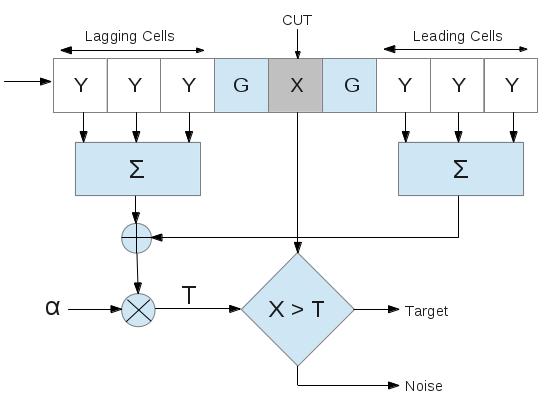
\includegraphics[width=3.5in]{../images/cacfar2.png}
\caption{Cell Averaging CFAR}
\label{fig:cfar}
\end{figure}

\par As you can see in figure \ref{fig:cfar}, the assumptions made when constructing even the simple CACFAR algorithm are the size of the leading and lagging windows, the number of guard cells, the scale factor $\alpha$ and the manner in which the comparison is carried out. In this example, a target which has energy spread across three or more cells will skew the summations and miss a detection. Many adaptations of this simple CFAR have been suggested to overcome the sensitivity of the summation by assuming a statistical distribution of the background cells or using order statistics \cite{sayed} \cite{shyam}. While these adaptations do provide better detection rates than the CACFAR in some cases they all still suffer from assuming a particular target size. For example, a target with high energy spread across the entire CFAR window will undoubtedly skew the statistics even when considering order statistics or a particular distribution.

\subsection{Modified CFAR using Morphological Operators}
\par To address the assumptions made in the CACFAR discussed above, we purpose a new algorithm not dependent on the sliding window. The new algorithm performs a search over the signal magnitude. This search will be performed using a global morphological watershed algorithm \cite[p.~769-776]{gonzalez}. The watershed algorithm performs multiple thresholds over the image in descending order (i.e. letting the water out of the catch basins). Any cells which exceed the watershed line will be considered a hypothesized detection. Adjacent cells in the 8 cell neighborhoods are then connected using a connected components algorithm to make a single region \cite[p.645-647]{gonzalez}. The regions are then enumerated, dilated and then the original regions are subtracted from the dilation to construct the "halo" of cells around the hypothesized detection. Background statistics are then computed for each of the regions using the surrounding cells in the halo. The background statistics are then compared to the statistics of the pixels in the hypothesized detected region. In keeping with the CACFAR, we compare the first moment of the background cells to the first moment of the region cells and record a detection if the contrast is greater. The background mean is multiplied by the user supplied gain factor as in the CACFAR described above. This comparison is computed for each threshold in the watershed algorithm. It is assumed that regions only increase in the number of cells, growing as the threshold of the watershed algorithm decreases. Therefore, hypothesized detected regions are tracked as the watershed algorithm continues. The final detected region consists of the region cells that had the largest contrast between the foreground and background.
\par To illustrate the algorithm, we will walk through an example using a one dimensional range profile extracted from a single cross-range bin of a SAR image shown in figure \ref{fig:sarhrr}. Due to the small amounts of energy scattered from most targets, the fidelity required to represent a RADAR signal is greater than 8-bits per pixel found in gray scale images. The dynamic range of a RADAR signal is often represented in IEEE 32-bit floating point precision. In order to perform a search of the signal using the watershed algorithm, the amplitude is quantized. We quantize the dynamic range of the signal by computing the histogram. The floating point precision of the bins and number of bins in the histogram is computed using the robust estimator known as Freedman-Diaconis rule \cite{freedman}. Using the histogram, we perform the watershed using the lower amplitude value associated with each histogram bin as the threshold. In effect, at each histogram bin, we are considering all the cells in the upper portion of the histogram. The watershed search is illustrated in figure \ref{fig:watershed}. The horizontal black lines in the figure represent the  thresholds of the watersheds. The green portions of the threshold line represent the hypothesized connected regions as detections. The red portions of the threshold line, drawn only on the largest return, show the background cells used during characterization. The background cells were chosen by dilating and subtracting the connected region.

\begin{figure}[!h]
\centering
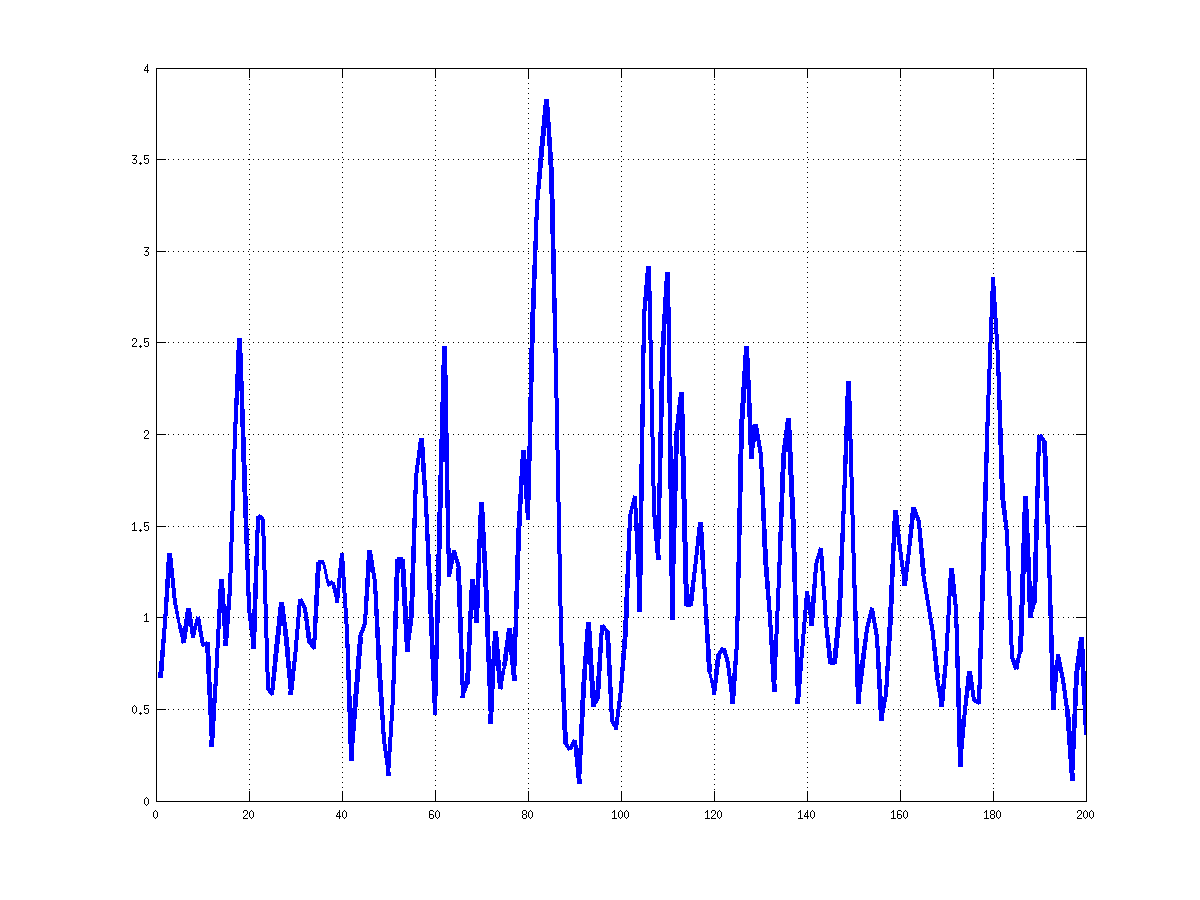
\includegraphics[width=3.75in]{../images/hrr.png}
\caption{Plot of Single Range Bin of SAR Image}
\label{fig:sarhrr}
\end{figure}

\begin{figure}[!h]
\centering
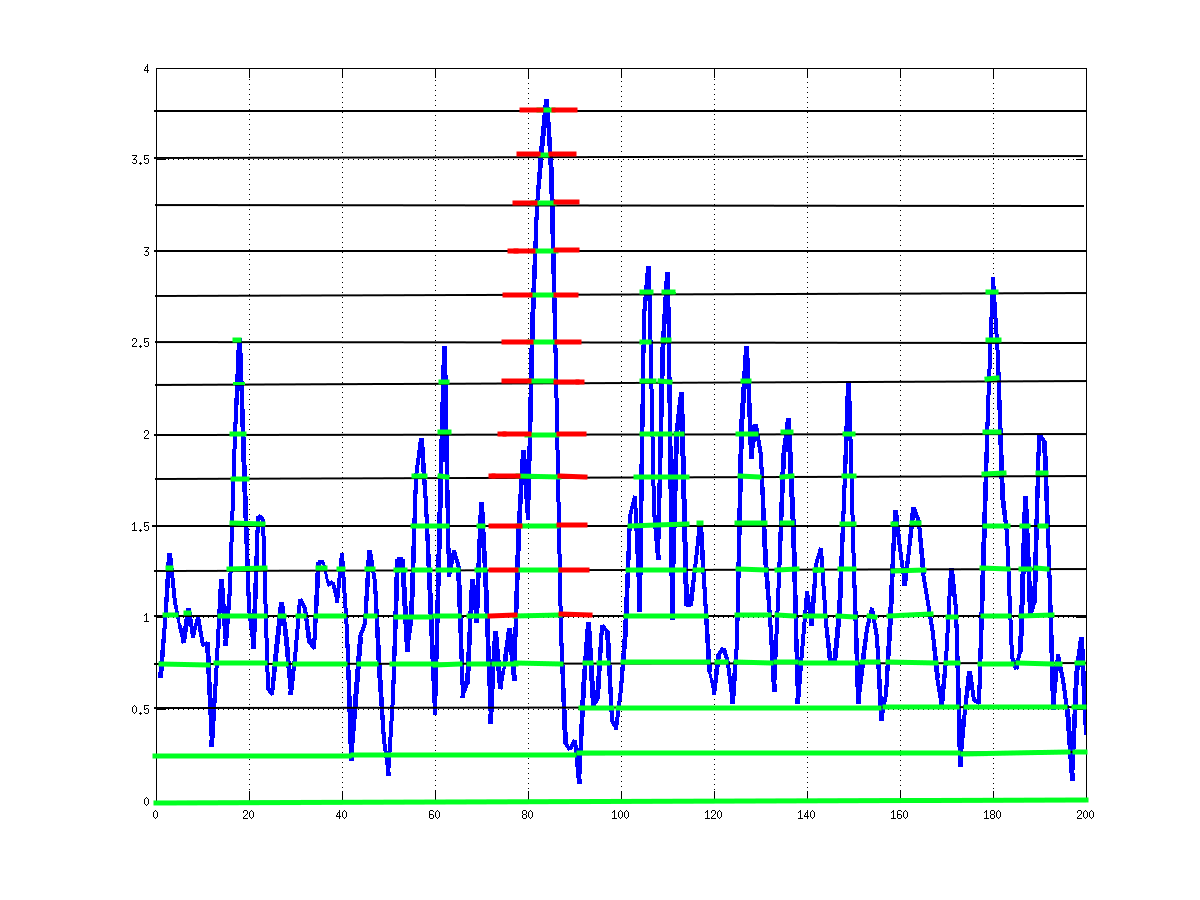
\includegraphics[width=3.75in]{../images/hrr_thresh.png}
\caption{Plot of Watershed Thresholds}
\label{fig:watershed}
\end{figure}

\par To further demonstrate the algorithm, we extend the example to the two dimensional SAR image in figure \ref{fig:starlite}. This image was acquired using the AN/ZPY-1 STARLite Small Tactical Radar by Northrop Grumman in strip-map collection mode \cite{northrop}. First, a slight image enhancement was performed on the image using a simple median filter to reduce the speckle and salt-and-pepper noise \cite[p.~156-157]{gonzalez}. The output of the median filter is in figure \ref{fig:starlite_median}. Then the quantized histogram was computed and applied to perform the watershed algorithm. Four thresholds of the watershed are illustrated in table \ref{tab:watershed}. Note, the top left image of the table shows well-formed detected regions with strong background support. For each threshold in the watershed, the connected components were computed form hypothesized detected regions. The halo of cells around each regions was computed via dilation and subtraction of the region cell pixels. Finally, the regions with the largest contrast of first moments between foreground and background were extracted. The output of this particular detection is shown in figure \ref{fig:starlite_detections}. The entire algorithm is detailed in figure \ref{fig:algorithm}.

\begin{figure}[!h]
\centering
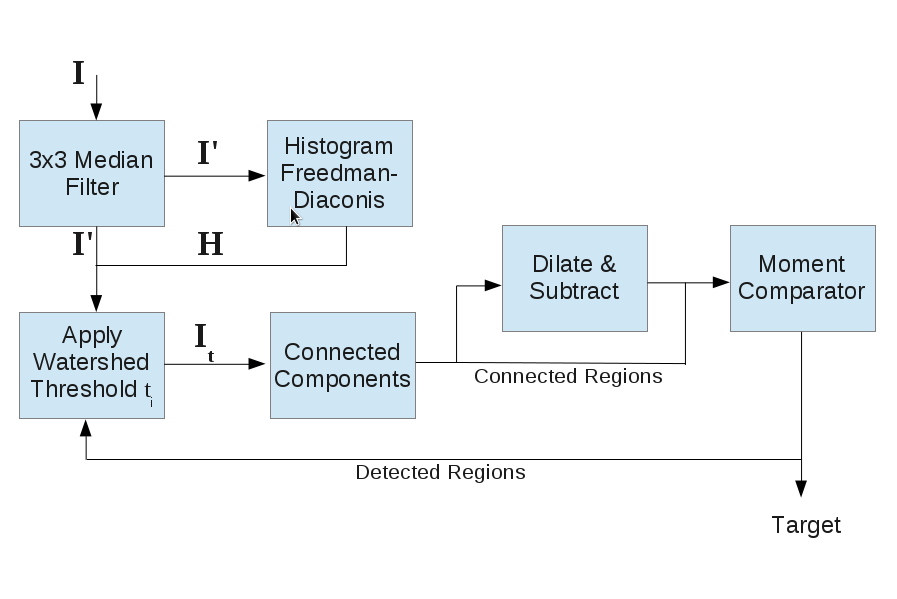
\includegraphics[width=3.75in]{../images/algorithm.png}
\caption{New Detection Logic}
\label{fig:algorithm}
\end{figure}


\begin{figure}[!h]
\centering
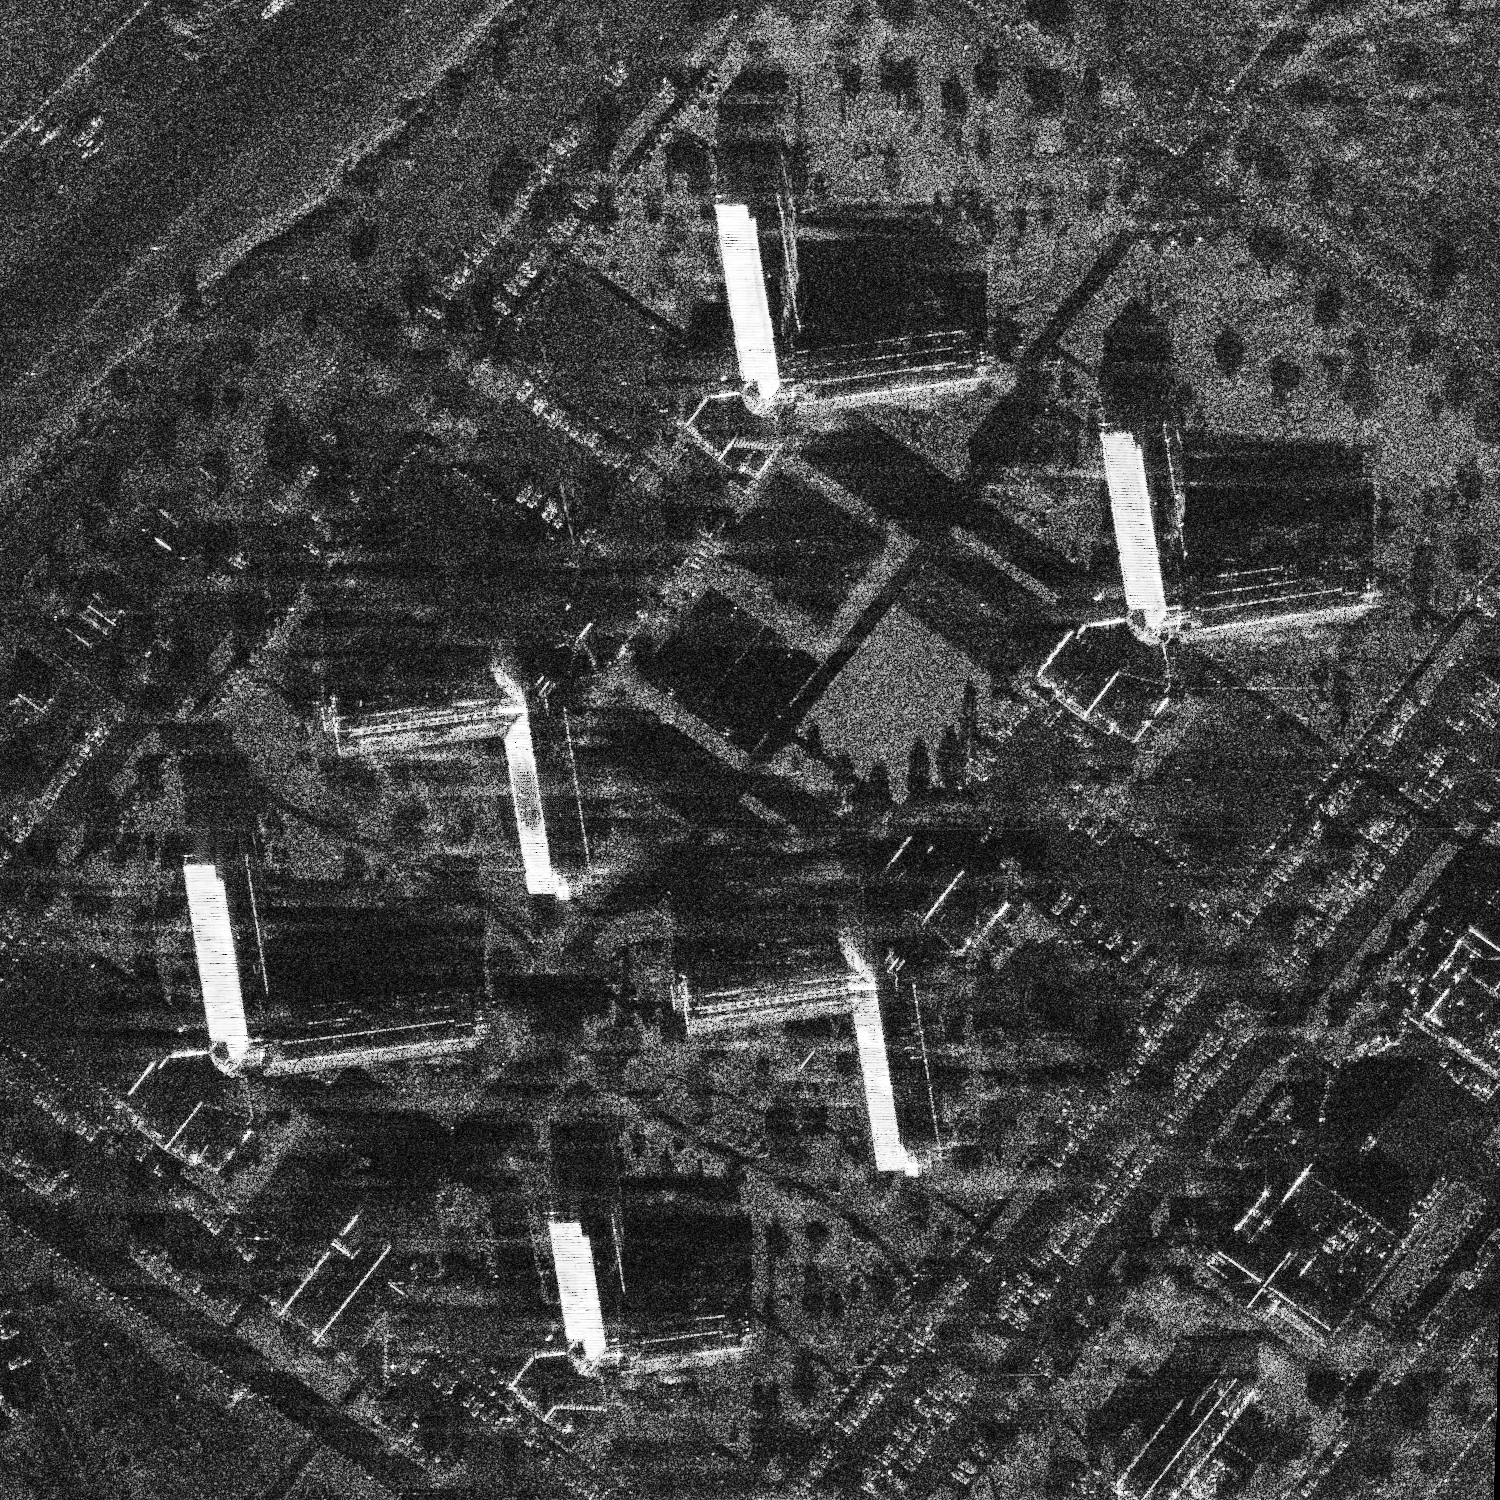
\includegraphics[width=3.0in]{../images/starlite_sar_lg.jpg}
\caption{Original Strip-Map SAR Image}
\label{fig:starlite}
\end{figure}

\begin{figure}[!h]
\centering
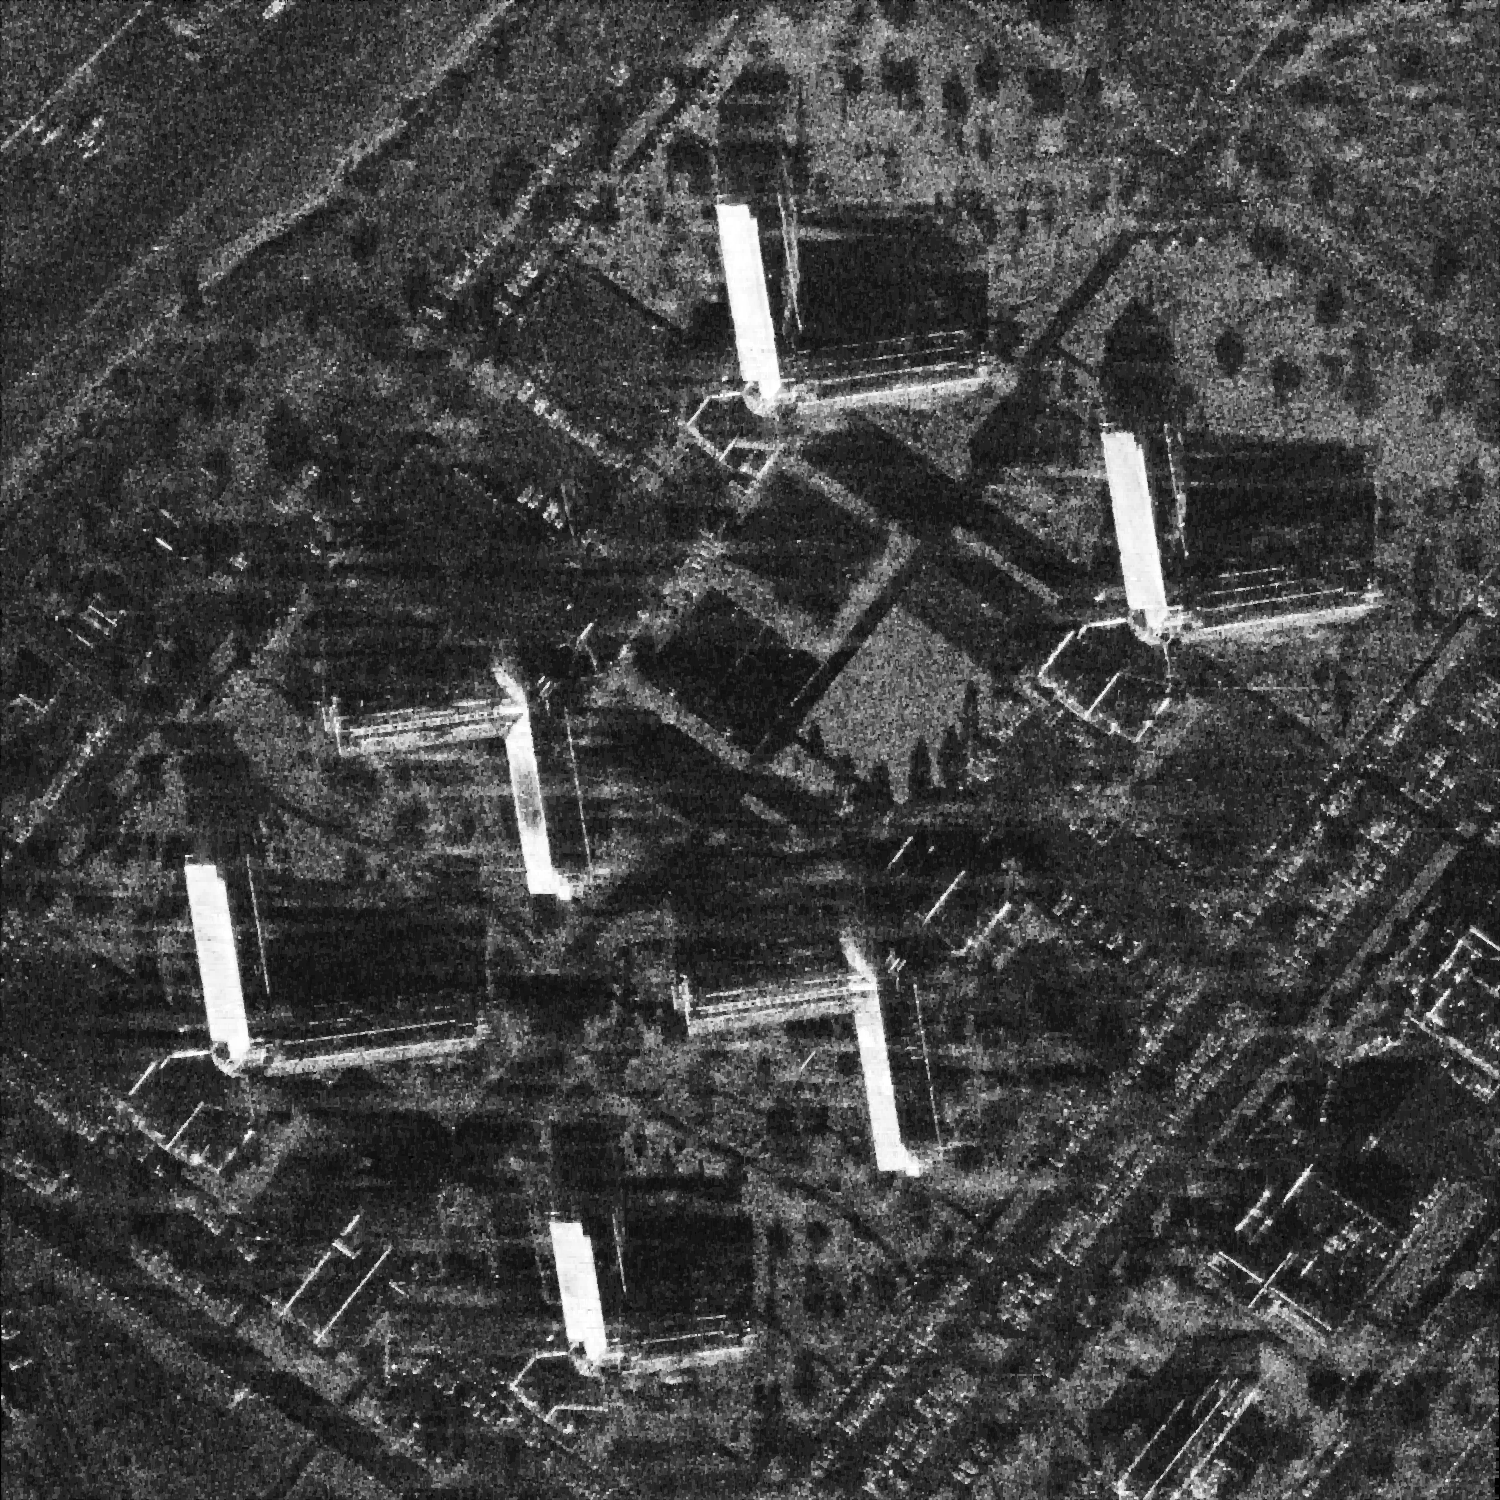
\includegraphics[width=3.0in]{../images/starlite_sar_lg_median.png}
\caption{Strip-Map SAR Image after Median Filter}
\label{fig:starlite_median}
\end{figure}

\begin{table}[!h]
\centering
\begin{tabular}{cc}
\includegraphics[width=1.5in]{../results/floodfills/floodfill_040.png} &
\includegraphics[width=1.5in]{../results/floodfills/floodfill_154.png} \\
\newline
\includegraphics[width=1.5in]{../results/floodfills/floodfill_230.png} &
\includegraphics[width=1.5in]{../results/floodfills/floodfill_300.png} \\
\end{tabular}
\caption{Four Thresholds of the Watershed Algorithm}
\label{tab:watershed}
\end{table}

\begin{figure}[!h]
\centering
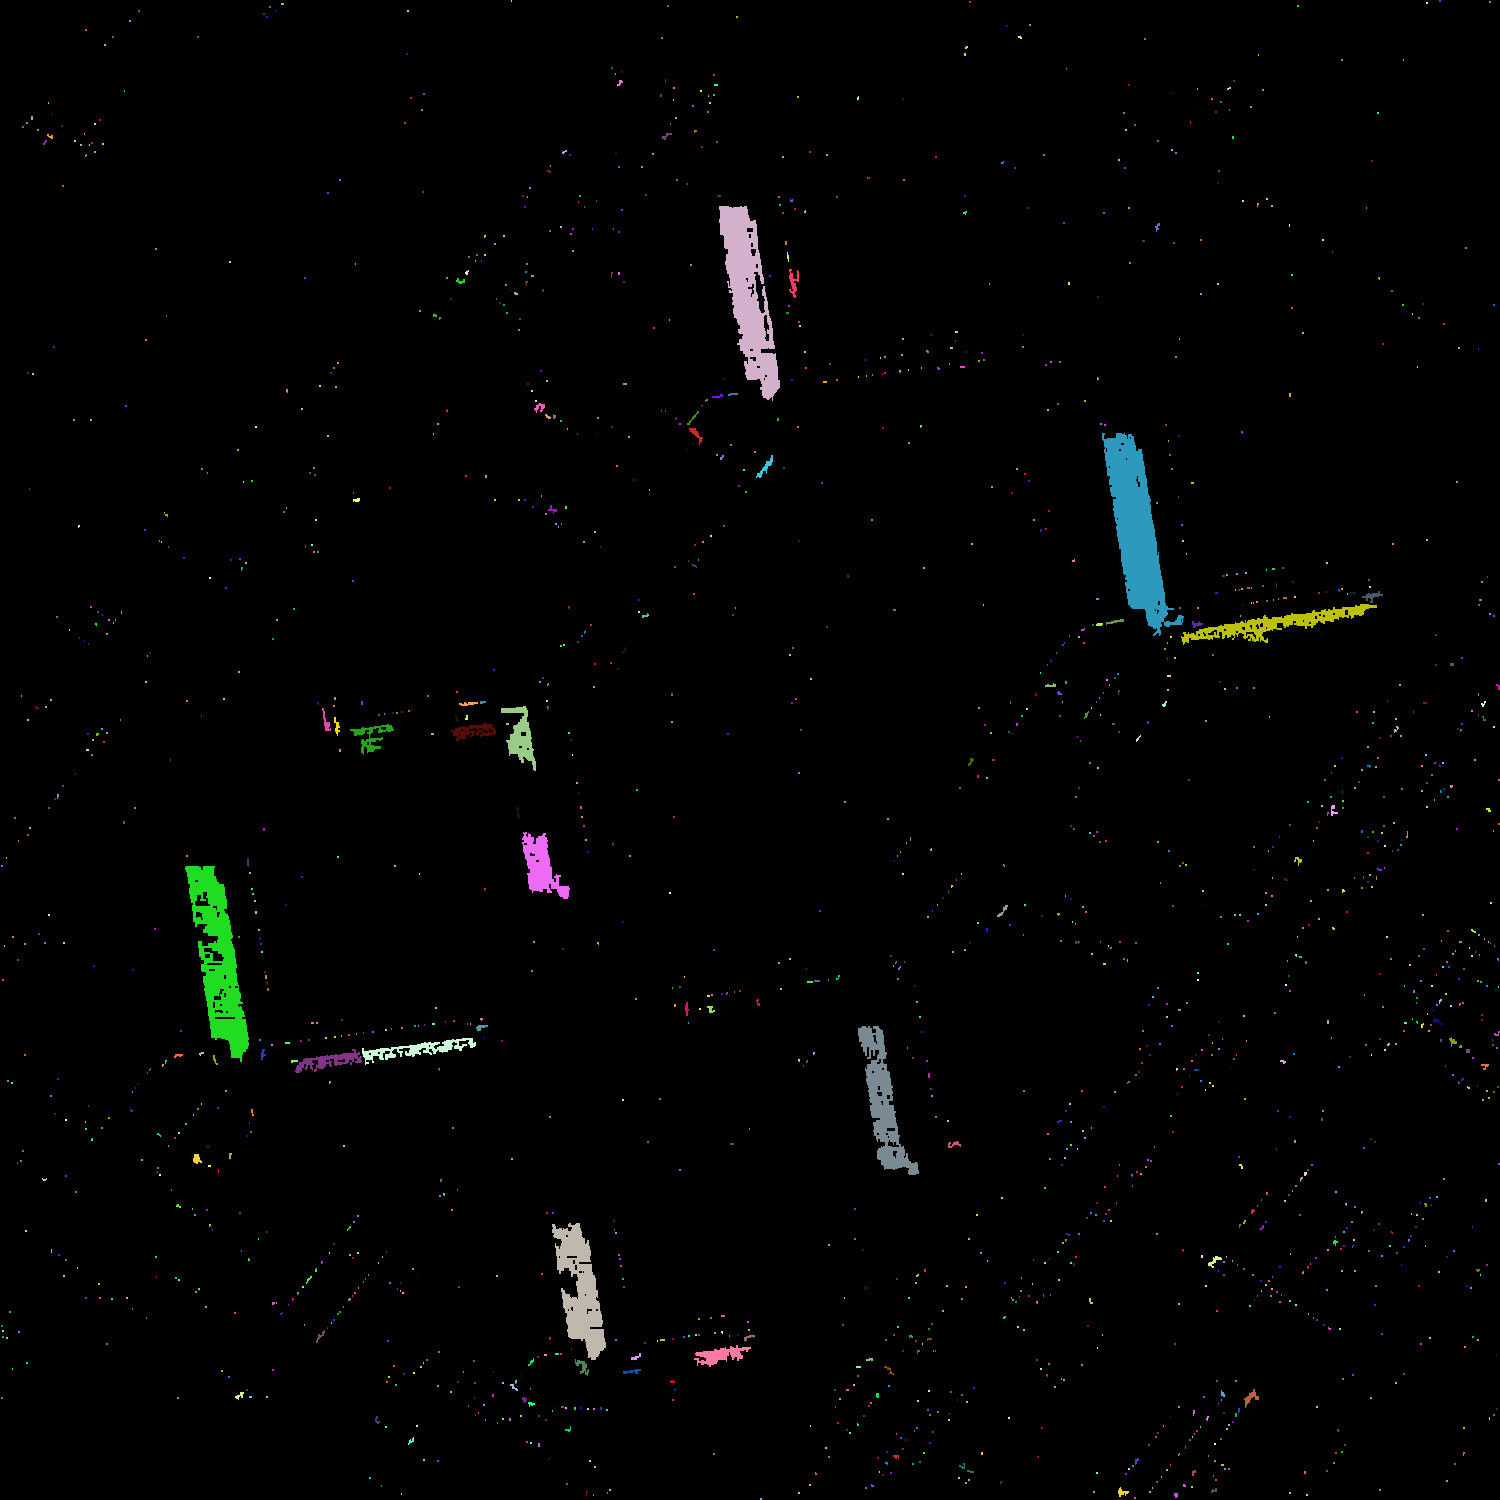
\includegraphics[width=3.0in]{../images/starlite_detections.png}
\caption{Connected Regions Detected from SAR Image}
\label{fig:starlite_detections}
\end{figure}


\subsection{Comparative Analysis of Detection Algorithms}
\par To compare the performance of the new algorithm versus the CACFAR on range extended target returns, we use a SAR image generated from a Sandia RADAR operating in the Ku-band with center frequency of 15 GHz. The image is shown in figure \ref{fig:sandia}. The detections found using the CACFAR algorithm are in figure \ref{fig:cfardetect}. The detections found using the watershed algorithm are in figure \ref{fig:mydetect}. It is clear that the CACFAR is inappropriate for this scene. The range extended target returns are not detected by the CACFAR due to the assumptions about scale built into the CFAR algorithm. The CACFAR is essentially saturated in the bright areas of the target return. The CACFAR did detect the point target returns in the courtyard, but failed entirely to detect the brightest returns. The assumptions of the CACFAR are overcome using the watershed algorithm as seen in figure \ref{fig:mydetect}.

\begin{figure}[!h]
\centering
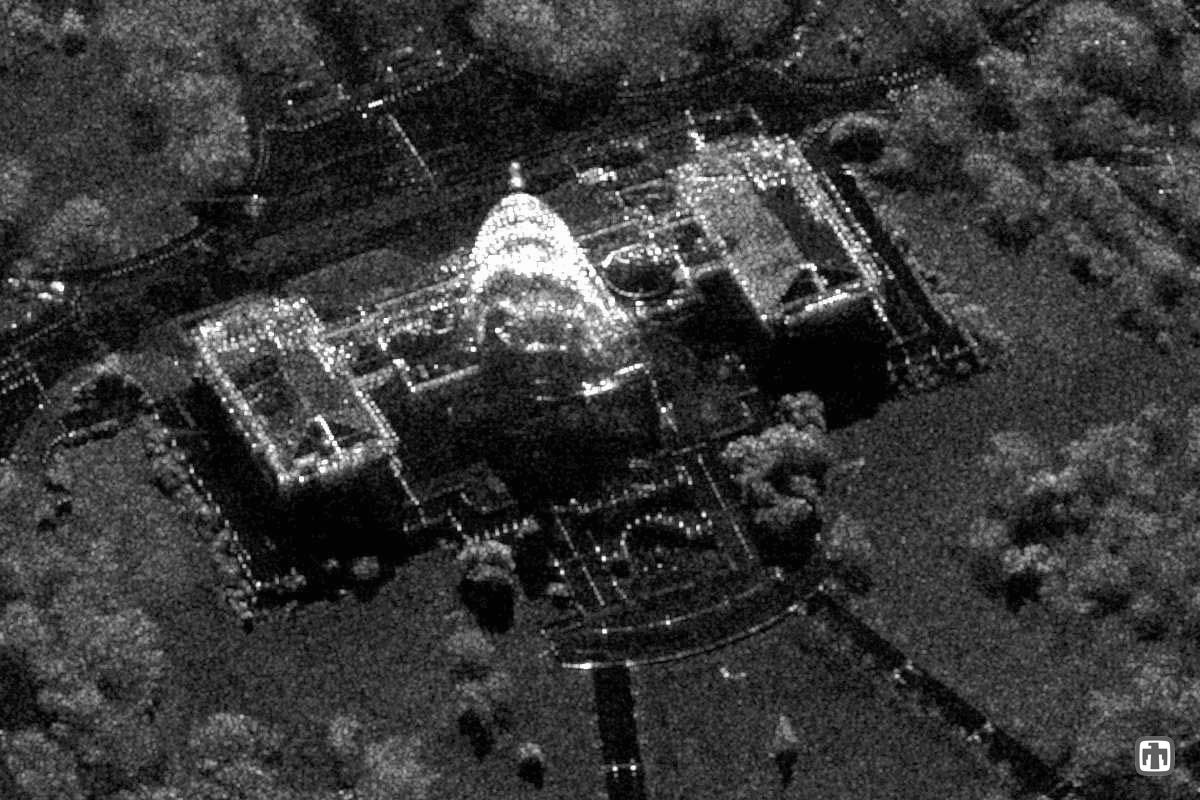
\includegraphics[width=3.0in]{../images/capitol.png}
\caption{Sandia Ku-Band SAR Image at 15 GHz}
\label{fig:sandia}
\end{figure}

\begin{figure}[!h]
\centering
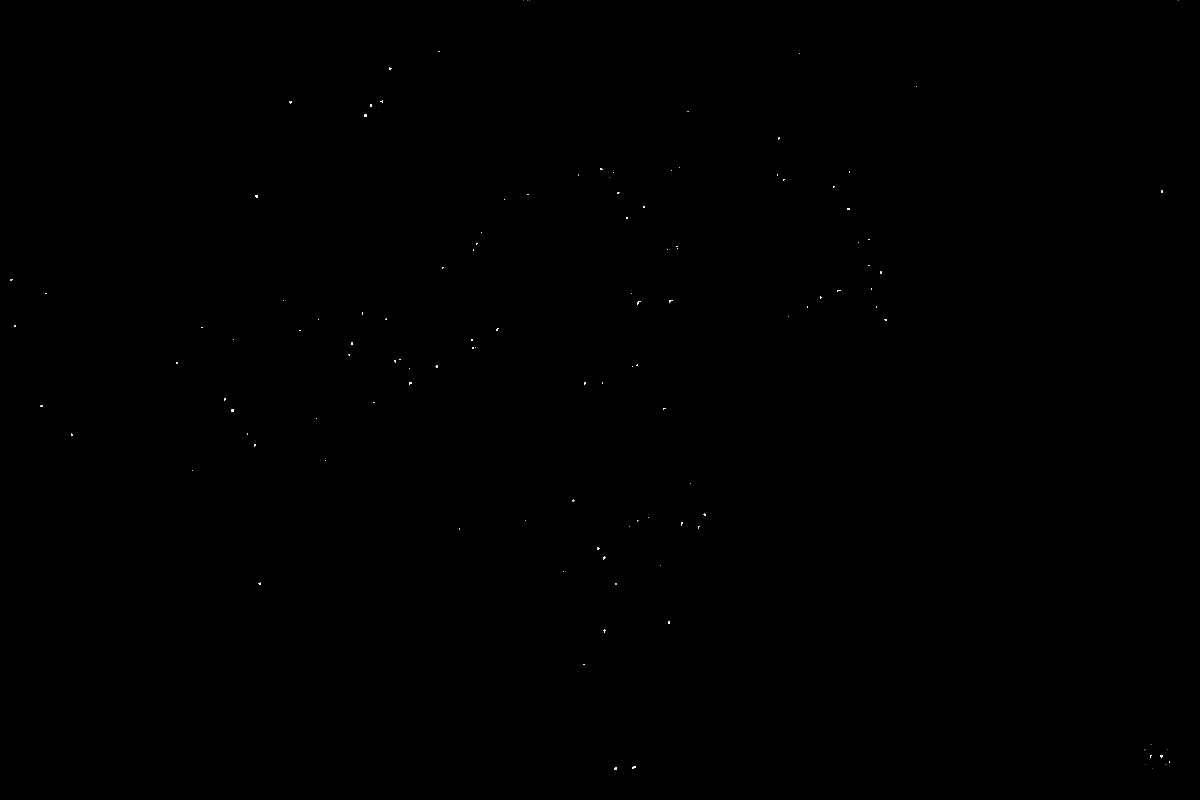
\includegraphics[width=3.0in]{../images/capitol_cfar.png}
\caption{CACFAR Detections of Sandia Image}
\label{fig:cfardetect}
\end{figure}

\begin{figure}[!h]
\centering
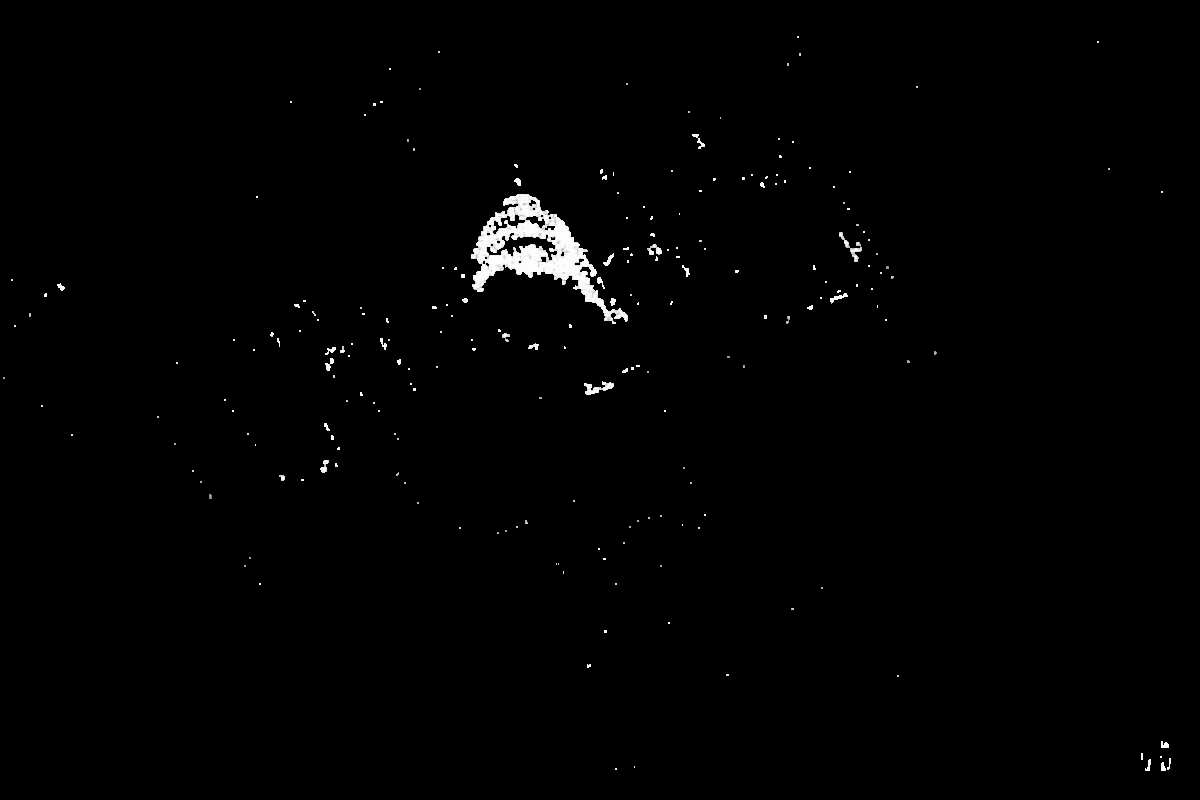
\includegraphics[width=3.0in]{../images/capitol_regions.png}
\caption{Watershed Detections of Sandia Image}
\label{fig:mydetect}
\end{figure}

\section{Conclusion}
In this paper, we have developed a new algorithm useful for detecting range extended target signatures in SAR imagery. The new detection algorithm does not perform a search over the time or spatial domain, but over the signal amplitude using a watershed threshold. The watershed allows the algorithm to choose the background pixels that provide the most supporting evidence for a detection. While this algorithm worked very well on range extended targets, the CACFAR outperformed this algorithm when detecting point targets of a known size in sparse environments. The application of the watershed algorithm is most appropriate in near field SAR and high resolution SAR imagery where scattered target energy is spread across multi-cell regions of the image.

% References section
\nocite{*}
\bibliographystyle{plain}
\bibliography{./references}

% Biography
\begin{IEEEbiographynophoto}{Bernard Lampe}
(M'09) became an IEEE Member (M) in 2009 and received his bachelors of science degree from The University of Michigan in Ann Arbor, Michigan, USA in 2009.
\par Mr. Lampe is also a member of the American Society for Computing Machines (ACM) since 2009.
\end{IEEEbiographynophoto}

% End document
\end{document}

